% Blok RTL SeBatt (Flow B) untuk spesifikasi.md bagian 2.
% Kompilasi: latexmk -pdf blok-rtl.tex
% PNG: pdftoppm -png -r 200 -singlefile blok-rtl.pdf blok-rtl
\documentclass[border=8pt]{standalone}
\usepackage[T1]{fontenc}
\usepackage[scaled=0.92]{helvet}
\renewcommand{\familydefault}{\sfdefault}
\usepackage{tikz}
\usetikzlibrary{positioning,arrows.meta,fit,backgrounds,calc}

\begin{document}
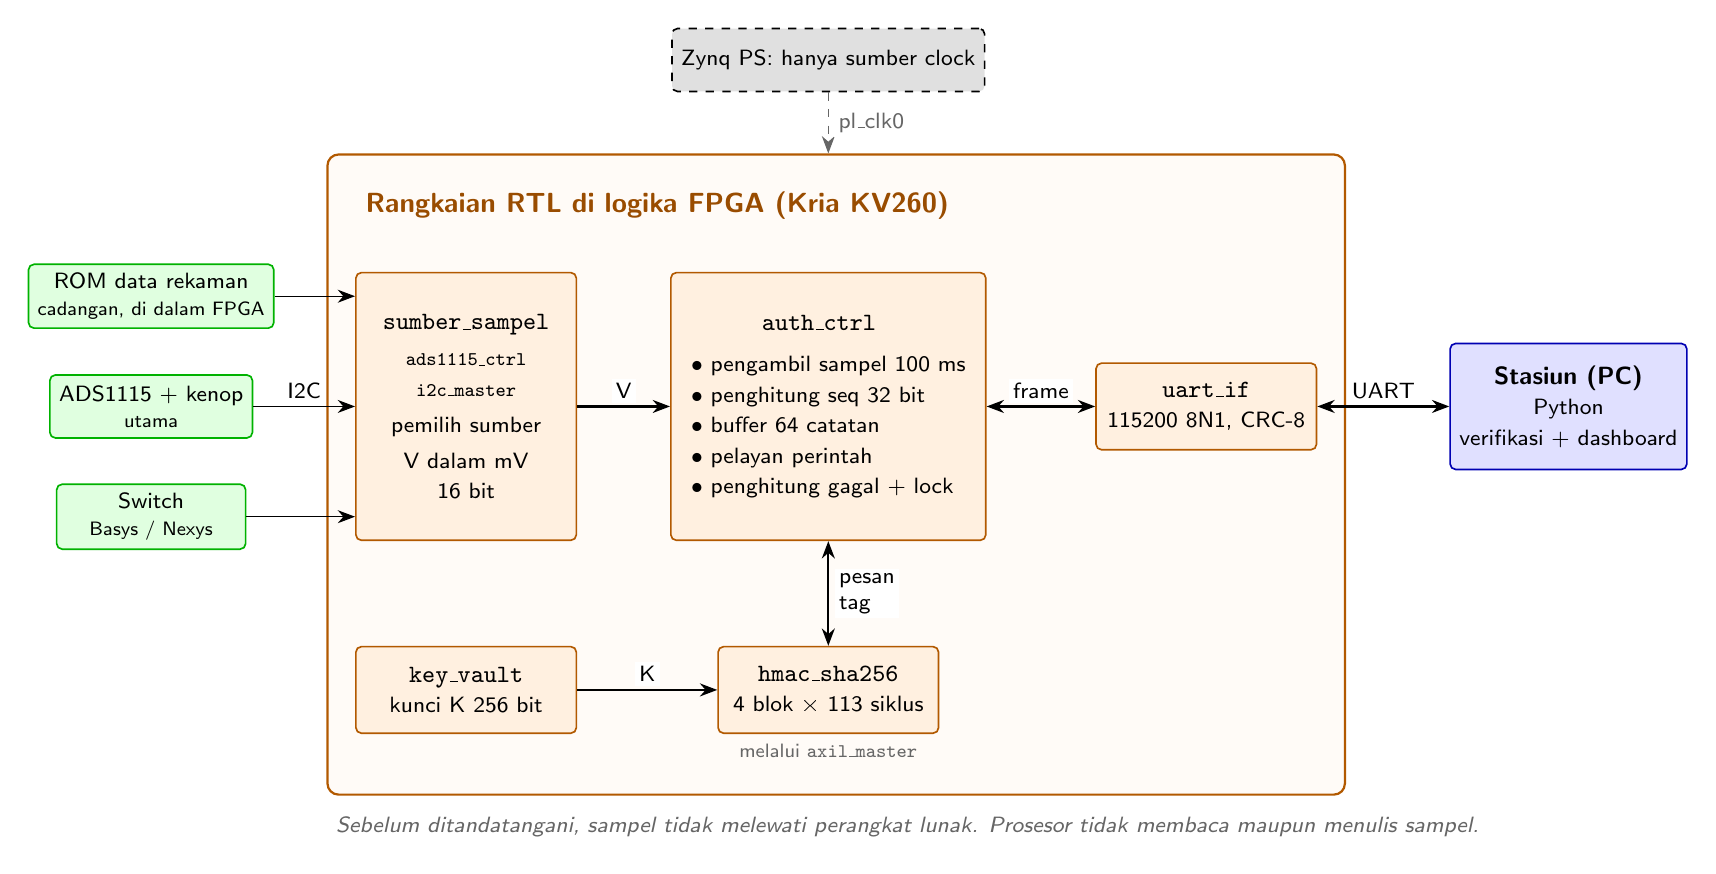
\begin{tikzpicture}[
    font=\small, >={Stealth[length=2.2mm]},
    blk/.style={draw=#1!70!black, fill=#1!12, rounded corners=2pt, align=center,
                minimum width=28mm, minimum height=11mm, line width=0.6pt},
    ip/.style={blk=orange},
    src/.style={blk=green, minimum width=24mm, minimum height=8mm, font=\footnotesize},
    lbl/.style={font=\footnotesize, fill=white, inner sep=1.5pt}
  ]

  % Sumber masukan di luar/di dalam FPGA
  \node[src] (rom) at (0,1.4)  {ROM data rekaman\\{\scriptsize cadangan, di dalam FPGA}};
  \node[src] (adc) at (0,0)    {ADS1115 + kenop\\{\scriptsize utama}};
  \node[src] (sw)  at (0,-1.4) {Switch\\{\scriptsize Basys / Nexys}};

  % IP di FPGA
  \node[ip, minimum height=34mm] (mux) at (4.0,0) {\texttt{sumber\_sampel}\\[2pt]{\scriptsize\texttt{ads1115\_ctrl}}\\{\scriptsize\texttt{i2c\_master}}\\[2pt]{\footnotesize pemilih sumber}\\[2pt]{\footnotesize V dalam mV}\\{\footnotesize 16 bit}};
  \node[ip, minimum width=40mm, minimum height=34mm, align=left] (ctrl) at (8.6,0)
    {\hspace*{9mm}\texttt{auth\_ctrl}\\[4pt]
     {\footnotesize $\bullet$ pengambil sampel 100 ms}\\
     {\footnotesize $\bullet$ penghitung seq 32 bit}\\
     {\footnotesize $\bullet$ buffer 64 catatan}\\
     {\footnotesize $\bullet$ pelayan perintah}\\
     {\footnotesize $\bullet$ penghitung gagal + lock}};
  \node[ip] (uart) at (13.4,0) {\texttt{uart\_if}\\{\footnotesize 115200 8N1, CRC-8}};
  \node[ip] (hmac) at (8.6,-3.6) {\texttt{hmac\_sha256}\\{\footnotesize 4 blok × 113 siklus}};
  \node[font=\scriptsize, text=black!60, anchor=north] (axl) at (hmac.south) {melalui \texttt{axil\_master}};
  \node[ip] (key)  at (4.0,-3.6) {\texttt{key\_vault}\\{\footnotesize kunci K 256 bit}};

  % Prosesor hanya sumber clock
  \node[blk=black, minimum width=34mm, minimum height=8mm, font=\footnotesize, dashed] (ps) at (8.6,4.4)
    {Zynq PS: hanya sumber clock};

  \node[font=\bfseries, text=orange!60!black, anchor=west] (lbl) at (2.6,2.55) {Rangkaian RTL di logika FPGA (Kria KV260)};
  \begin{scope}[on background layer]
    \node[draw=orange!70!black, fill=orange!3, rounded corners=4pt, line width=0.8pt,
          inner sep=3.5mm, fit=(mux)(ctrl)(uart)(hmac)(key)(lbl)(axl)] (fpga) {};
  \end{scope}

  % Stasiun
  \node[blk=blue, minimum width=30mm, minimum height=16mm] (pc) at (18.0,0)
    {\textbf{Stasiun (PC)}\\{\footnotesize Python}\\{\footnotesize verifikasi + dashboard}};

  % Panah
  \draw[->] (rom.east) -- (mux.west |- rom.east);
  \draw[->] (adc.east) -- node[lbl, above=1pt]{I2C} (mux.west |- adc.east);
  \draw[->] (sw.east)  -- (mux.west |- sw.east);
  \draw[->, line width=0.8pt] (mux) -- node[lbl, above=1pt]{V} (ctrl);
  \draw[<->, line width=0.8pt] (ctrl) -- node[lbl, above=1pt]{frame} (uart);
  \draw[<->, line width=0.8pt] (uart) -- node[lbl, above=1pt]{UART} (pc);
  \draw[<->, line width=0.8pt] (ctrl) -- node[lbl, right=2pt, align=left]{pesan\\tag} (hmac);
  \draw[->, line width=0.8pt] (key) -- node[lbl, above=1pt]{K} (hmac);
  \draw[->, dashed, black!60] (ps) -- node[lbl, right=2pt]{pl\_clk0} (fpga.north -| ps);

  % Keterangan aturan jalur data
  \node[font=\footnotesize\itshape, text=black!60, anchor=north west, align=left]
    at ($(fpga.south west)+(0,-0.15)$)
    {Sebelum ditandatangani, sampel tidak melewati perangkat lunak. Prosesor tidak membaca maupun menulis sampel.};

\end{tikzpicture}
\end{document}
